\section{Experiments and Deep Diagnostics}
\label{sec:experiments}

We evaluate our framework across six research questions under strictly causal, leakage-free real-token accounting:
\begin{itemize}
    \item \textbf{RQ1 (Pareto Efficiency):} Across $20\text{k}/40\text{k}/80\text{k}$ real-token caps on development streams, how does mesoscopic querying compare with post- and edge-level active strategies?
    \item \textbf{RQ2 (Strictly Causal Held-Out Benchmark):} Across all $27$ unseen chronological held-out blocks in English and French, how does \texttt{SUG-Meso} compare against zero-LLM baselines, \texttt{Cequel-Transitive}, multi-seed \texttt{Random}, and \texttt{Random-Meso} under uncontaminated \texttt{all\_shown} $U_t$?
    \item \textbf{RQ3 (Structural Ablations \& Eq.~(5)/(6) Sensitivity):} What is the isolated role of each structural term in Eq.~\eqref{eq:u_merge} and Eq.~\eqref{eq:u_seam}, and how sensitive is \texttt{SUG-Meso} to merge/seam ratios and conductance thresholds?
    \item \textbf{RQ4 (Longitudinal Cross-Day Tracking):} Why did initial \texttt{SUG-CrossLLM-v1} trail unsupervised prototypes, and does \texttt{SUG-CrossLLM-v2} surpass all prototype thresholds across multi-week streams?
    \item \textbf{RQ5 (Anti-Memorization Stress Test):} Do gains vanish when $99.7\%$--$100\%$ of named entities, hashtags, and years are anonymized across all $27$ held-out blocks?
    \item \textbf{RQ6 (Confusion, Runtime, \& Failure Root Causes):} Where do remaining errors occur at the individual query level?
\end{itemize}

\subsection{Experimental Setup and Strictly Causal Protocol}
\label{sec:setup}

\paragraph{Chronological Benchmarks and Dev-Only Calibration.}
We evaluate on two chronological Twitter benchmarks (Table~\ref{tab:datasets}): \textbf{Event2012}~\citep{mcminn2013building} ($68{,}841$ English tweets, $503$ events across $22$ daily blocks) and \textbf{Event2018}~\citep{mazoyer2020french} ($64{,}516$ French tweets, $257$ events across $17$ blocks), merging days with fewer than $200$ posts after the initial $7$-day window $M_{00}$. Blocks $M_{00}$--$M_{01}$ initialize longitudinal memory at $0$ tokens, $M_{02}$--$M_{05}$ serve exclusively for development tuning, and $M_{06}+$ ($27$ held-out blocks totaling $65{,}856$ posts) remain strictly isolated during calibration.

\begin{table}[t]
\centering
\caption{Chronological dataset partitions across warmup, development, and $27$ unseen held-out blocks ($65{,}856$ evaluated posts).}
\label{tab:datasets}
\resizebox{\linewidth}{!}{%
\begin{tabular}{l|cc|ccc}
\toprule
\textbf{Split} & \textbf{Blocks} & \textbf{Dates} & \textbf{Posts} & \textbf{Events} & \textbf{Role} \\
\midrule
\multicolumn{6}{c}{\textbf{Event2012} (English, \texttt{all-MiniLM-L6-v2})} \\
\midrule
Warmup ($M_{00}$--$M_{01}$) & 2 & Oct 10--17, 2012 & 28,976 & 165 & Memory seed ($0$ tok) \\
Dev ($M_{02}$--$M_{05}$) & 4 & Oct 18--21, 2012 & 7,170 & 82 & Calibration \& $20\text{k}$--$80\text{k}$ curves \\
Held-Out ($M_{06}$--$M_{21}$) & 16 & Oct 22--Nov 7, 2012 & 32,695 & 292 & Causal held-out suite \\
\midrule
\multicolumn{6}{c}{\textbf{Event2018} (French, \texttt{paraphrase-multilingual-MiniLM-L12-v2})} \\
\midrule
Warmup ($M_{00}$--$M_{01}$) & 2 & Jul 16--23, 2018 & 19,684 & 89 & Memory seed ($0$ tok) \\
Dev ($M_{02}$--$M_{05}$) & 4 & Jul 24--27, 2018 & 11,671 & 51 & Calibration \& $20\text{k}$--$80\text{k}$ curves \\
Held-Out ($M_{06}$--$M_{16}$) & 11 & Jul 28--Aug 7, 2018 & 33,161 & 144 & Causal held-out suite \\
\bottomrule
\end{tabular}}
\end{table}

\paragraph{Unbiased Dev Prompt Selection and Causal LLM Setup.}
All Stage~2A/2B held-out experiments run \texttt{Qwen/Qwen3-8B}~\citep{yang2025qwen3} in deterministic non-thinking JSON mode (\texttt{enable\_thinking=False}, \texttt{temperature=0.0}, $0$ reasoning tokens), while Dev ($40\text{k}$) additionally tests \texttt{Llama-3.1-8B-Instruct}~\citep{grattafiori2024llama3}. Calibrating purely on Dev ($M_{02}$--$M_{05}$) under \texttt{CausalUniformFixed} ($10\text{k}$/blk): on \texttt{Event2012}, \texttt{Action-First} improves Dev AMI from $91.65$ to \textbf{$93.67$} (Macro-$B^3$ $70.72 \to 71.58$, Micro-$B^3$ $88.26 \to 91.87$, \texttt{MERGE} recall $0.6000 \to 0.8889$); on \texttt{Event2018}, \texttt{Action-First} improves Dev AMI from $72.22$ to \textbf{$75.49$} (Macro-$B^3$ $69.19 \to 70.89$, Micro-$B^3$ $68.72 \to 76.18$, \texttt{MERGE} recall $0.5000 \to 0.8750$). Accordingly, \texttt{Action-First} is pre-selected without touching held-out data, while both prompt schemas are reported side by side for transparency. Statistical significance across blocks uses paired two-sided Wilcoxon signed-rank tests~\citep{wilcoxon1945individual} with Holm-Bonferroni correction~\citep{holm1979simple} and paired effect size Cohen's $d_z$~\citep{cohen1988statistical}.

\paragraph{Zero-LLM and Same-Budget Comparators.}
On identical graphs and initial partitions $\mathcal{P}_t^{(0)}$, we benchmark: (i)~\textbf{0-LLM baselines}: \texttt{Init 2D-SE}~\citep{cao2024hisevent}, \texttt{Vanilla 2D-SE} (without node-move refinement), \texttt{Semantic-Only 2D-SE} ($\alpha=0$), \texttt{Dev-Tuned 2D-SE} (grid-tuned $\tau_{\text{sim}}=0.45$, $\alpha=0.5$/$0.8$ on Dev), \texttt{Louvain}~\citep{blondel2008fast} (Dev-tuned resolution $1.2$ EN / $0.5$ FR), \texttt{Agglom-Cosine}~\citep{pedregosa2011scikit} ($d=0.55$), and \texttt{Meso-Heur (0-Tok)} (identical \texttt{MERGE\_PAIR}/\texttt{SPLIT\_SEAM} candidates thresholded purely by Dev-tuned cosines $\tau_m=0.80$ EN / $0.75$ FR); and (ii)~\textbf{same-budget LLM baselines}: $3$-seed \texttt{Random} (seeds $42,100,200$), \texttt{Rep-Div} (MMR~\citep{liu2026ragsede}), \texttt{Cequel-Edge}~\citep{wang2025cequel} (\texttt{Direct}/\texttt{Repair}), \texttt{Cequel-Transitive} (cluster-level transitive union-find with cannot-link guards), and $3$-seed \texttt{Random-Meso} (identical $65\%/35\%$ \texttt{MERGE\_PAIR}/\texttt{SPLIT\_SEAM} structure in random order).

\begin{figure*}[t]
  \centering
  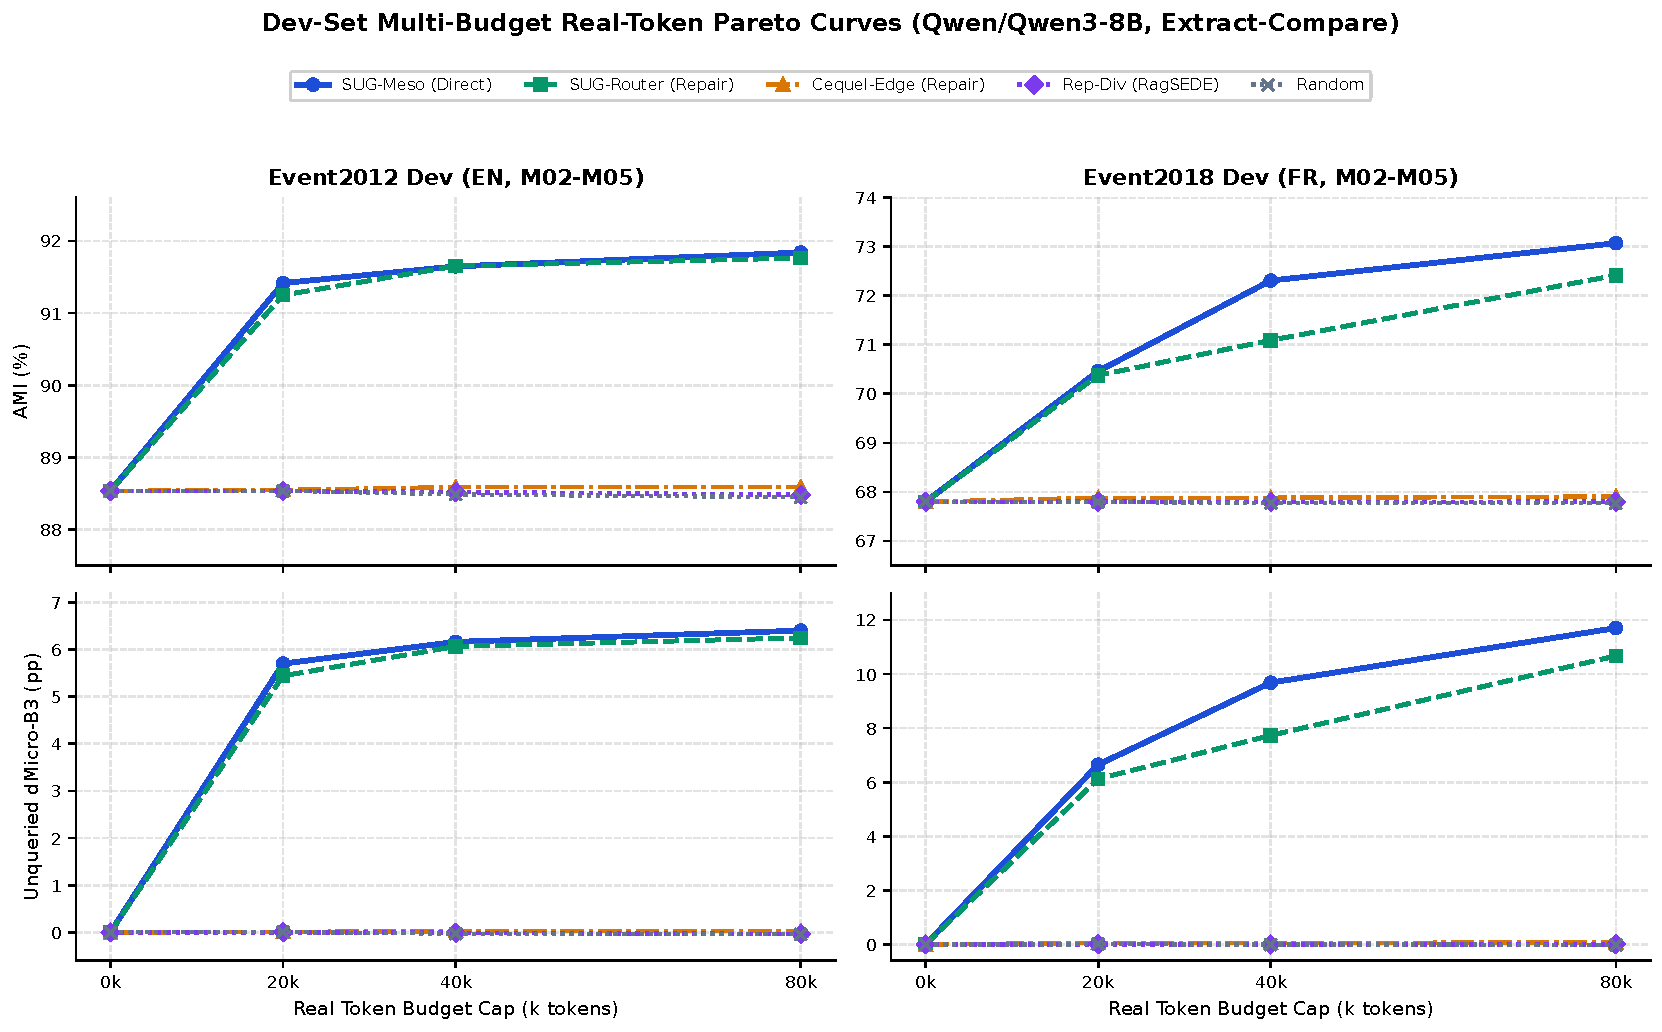
\includegraphics[width=\textwidth]{figures/fig_budget_pareto.pdf}
  \caption{Multi-budget real-token Pareto curves across $\{0, 20\text{k}, 40\text{k}, 80\text{k}\}$ tokens (prompt + completion) on \texttt{Event2012} and \texttt{Event2018} dev blocks (\texttt{Qwen/Qwen3-8B}, $1{,}147/1{,}147$ zero-error calls). At $20\text{k}$ tokens ($7$--$9$ calls/block), \texttt{SUG-Meso} surpasses all post- and pair-level baselines given $80\text{k}$ tokens ($4\times$ budget).}
  \label{fig:budget_curves}
\end{figure*}

\subsection{RQ1: Multi-Budget Real-Token Pareto Curves}
\label{sec:rq1}
Figure~\ref{fig:budget_curves} and Table~\ref{tab:budget_dev} vary cumulative token caps across $\{0, 20\text{k}, 40\text{k}, 80\text{k}\}$ on Dev ($M_{02}$--$M_{05}$), completing $1{,}147/1{,}147$ calls with zero errors:
\begin{enumerate}
    \item \textbf{$4\times$ Pareto Dominance:} At $20\text{k}$ tokens ($\sim 5\text{k}$/block), \texttt{SUG-Meso (Direct)} achieves $+2.88\text{ pp}$ AMI and $+5.70\text{ pp}$ Unqueried Micro-$B^3$ on \texttt{Event2012}, and $+2.66\text{ pp}$ AMI / $+6.65\text{ pp}$ Unqueried Micro-$B^3$ on \texttt{Event2018}, whereas \texttt{Random}, \texttt{Rep-Div}, and \texttt{Cequel-Edge} move at most $+0.11\text{ pp}$ AMI even at $80\text{k}$ tokens.
    \item \textbf{Natural Saturation \& Cross-Lingual Scaling:} On \texttt{Event2012}, \texttt{SUG-Meso} exhausts all candidate mesoscopic seams at $61{,}344$ tokens ($91.84$ AMI), saving unused budget, while on \texttt{Event2018} it climbs monotonically across $20\text{k} \to 40\text{k} \to 80\text{k}$ to reach $73.07$ AMI ($+5.28\text{ pp}$), $69.30$ Macro-$B^3$ ($+4.81\text{ pp}$), and $+11.70\text{ pp}$ Unqueried Micro-$B^3$.
    \item \textbf{Dev Generalization on \texttt{Llama-3.1-8B-Instruct}:} Under $40\text{k}$ tokens on \texttt{Event2012} Dev, \texttt{Llama-3.1-8B-Instruct} reproduces the gap (\texttt{SUG-Router Direct} $+2.75\text{ pp}$ AMI vs.\ $\le +0.05\text{ pp}$ for \texttt{Rep-Div}/\texttt{Cequel}), while exposing a key cross-family framing contrast: naive \texttt{Action-First} induces severe yes-bias ($-36{,}684$ net False Merge change, $-4.17\text{ pp}$ Macro-$B^3$), which \texttt{Extract-Then-Compare} eliminates ($12/12 = 100\%$ \texttt{MERGE} precision).
\end{enumerate}

\begin{table}[t]
\centering
\caption{Dev-set Pareto benchmark on \texttt{Event2012} (Init AMI $88.53$, Mac-$B^3$ $69.17$) and \texttt{Event2018} (Init AMI $67.80$, Mac-$B^3$ $64.49$) across real-token tiers ($\times 100$ except tokens).}
\label{tab:budget_dev}
\resizebox{\linewidth}{!}{%
\begin{tabular}{c|l|rrr|rrr}
\toprule
 &  & \multicolumn{3}{c|}{\textbf{Event2012 Dev ($M_{02}$--$M_{05}$)}} & \multicolumn{3}{c}{\textbf{Event2018 Dev ($M_{02}$--$M_{05}$)}} \\
\textbf{Cap} & \textbf{Method} & \textbf{Tok} & \textbf{AMI ($\Delta$)} & \textbf{Mac ($\Delta$)} & \textbf{Tok} & \textbf{AMI ($\Delta$)} & \textbf{Mac ($\Delta$)} \\
\midrule
\multirow{5}{*}{20k}
 & Random (Dir) & 18,766 & 88.54 (+0.00) & 69.18 (+0.00) & 18,030 & 67.79 (-0.00) & 64.50 (+0.00) \\
 & Rep-Div (Dir) & 18,155 & 88.53 (-0.00) & 69.17 (-0.00) & 18,940 & 67.80 (+0.00) & 64.49 (+0.00) \\
 & Cequel (Rep) & 19,458 & 88.55 (+0.01) & 69.18 (+0.00) & 18,687 & 67.88 (+0.08) & 64.93 (+0.44) \\
 & SUG-Router (Rep) & 19,334 & 91.25 (+2.72) & 70.48 (+1.31) & 19,060 & 70.38 (+2.58) & \textbf{67.24 (+2.75)} \\
 & SUG-Meso (Dir) & 19,540 & \textbf{91.42 (+2.88)} & \textbf{70.91 (+1.73)} & 18,371 & \textbf{70.46 (+2.66)} & 67.02 (+2.53) \\
\midrule
\multirow{4}{*}{40k}
 & Cequel (Rep) & 39,582 & 88.59 (+0.05) & 69.20 (+0.03) & 39,085 & 67.88 (+0.08) & 64.93 (+0.44) \\
 & SUG-Router (Rep) & 39,185 & \textbf{91.65 (+3.12)} & \textbf{71.42 (+2.24)} & 39,413 & 71.09 (+3.29) & 68.11 (+3.62) \\
 & SUG-Meso (Dir) & 39,313 & \textbf{91.65 (+3.11)} & 70.72 (+1.55) & 38,808 & \textbf{72.31 (+4.51)} & \textbf{69.20 (+4.71)} \\
 & SUG-Meso (Rep) & 39,313 & \textbf{91.65 (+3.11)} & 70.72 (+1.55) & 38,808 & 72.19 (+4.39) & 68.68 (+4.19) \\
\midrule
\multirow{5}{*}{80k}
 & Random (Dir) & 77,923 & 88.44 (-0.09) & 69.11 (-0.07) & 77,999 & 67.76 (-0.03) & 64.57 (+0.08) \\
 & Rep-Div (Dir) & 77,511 & 88.48 (-0.05) & 69.06 (-0.11) & 78,475 & 67.80 (+0.01) & 64.52 (+0.03) \\
 & Cequel (Rep) & 79,728 & 88.59 (+0.05) & 69.20 (+0.03) & 78,497 & 67.91 (+0.11) & 64.94 (+0.44) \\
 & SUG-Router (Rep) & 79,281 & 91.76 (+3.23) & \textbf{71.53 (+2.36)} & 78,303 & 72.42 (+4.62) & 68.80 (+4.31) \\
 & SUG-Meso (Dir) & 61,344 & \textbf{91.84 (+3.31)} & 70.89 (+1.72) & 78,821 & \textbf{73.07 (+5.28)} & \textbf{69.30 (+4.81)} \\
\bottomrule
\end{tabular}}
\end{table}

\subsection{RQ2: Strictly Causal Held-Out Benchmark \& Uncontaminated $U_t$}
\label{sec:rq2}

\begin{table*}[t]
\centering
\caption{Strictly causal held-out evaluation across $27$ unseen chronological blocks ($32{,}695$ EN + $33{,}161$ FR tweets) under uncontaminated \texttt{all\_shown} $U_t$ ($100\%$ zero-error ledgers across all $38$ Stage~2A within-block runs $\times 2$ datasets). Values are $\times 100$ except Show\%, Tok/post, and UnqNet.}
\label{tab:heldout_main}
\resizebox{\textwidth}{!}{%
\begin{tabular}{l|cccccc|cccccc}
\toprule
 & \multicolumn{6}{c|}{\textbf{Event2012 Held-Out ($M_{06}$--$M_{21}$, 16 blocks)}} & \multicolumn{6}{c}{\textbf{Event2018 Held-Out ($M_{06}$--$M_{16}$, 11 blocks)}} \\
\textbf{Method / Controller} & \textbf{Show\%} & \textbf{AMI} & \textbf{Mac-$B^3$} & \textbf{Tail-$B^3$} & \textbf{Unq $\Delta$Mic} & \textbf{UnqNet} & \textbf{Show\%} & \textbf{AMI} & \textbf{Mac-$B^3$} & \textbf{Tail-$B^3$} & \textbf{Unq $\Delta$Mic} & \textbf{UnqNet} \\
\midrule
Init 2D-SE (0-Tok) & 0.00 & 83.95 & 65.67 & 41.03 & --- & --- & 0.00 & 76.34 & 67.90 & 35.00 & --- & --- \\
Vanilla 2D-SE (no moves) & 0.00 & 83.95 & 65.35 & 40.90 & --- & --- & 0.00 & 76.71 & 67.68 & 35.26 & --- & --- \\
Semantic-Only 2D-SE ($\alpha=0$) & 0.00 & 84.16 & 64.82 & 38.98 & --- & --- & 0.00 & 75.66 & 62.86 & 21.76 & --- & --- \\
Dev-Tuned 2D-SE (0-Tok) & 0.00 & 84.17 & 73.68 & 60.92 & --- & --- & 0.00 & 75.64 & 70.00 & 43.76 & --- & --- \\
Louvain (Dev res.) & 0.00 & 84.46 & 54.71 & 23.19 & --- & --- & 0.00 & 81.11 & 53.61 & 7.89 & --- & --- \\
Agglom-Cosine ($d=0.55$) & 0.00 & 85.62 & \textbf{76.52} & \textbf{70.91} & --- & --- & 0.00 & 69.90 & 73.01 & \textbf{75.18} & --- & --- \\
Meso-Heur (0-Tok) & 0.00 & 88.36 & 66.86 & 40.85 & --- & --- & 0.00 & 81.49 & 70.86 & 36.78 & --- & --- \\
\midrule
Random (3-seed Mean) & 3.69 & 83.91 & 65.79 & 41.36 & -0.03 & -62.2 & 2.06 & 76.32 & 67.95 & 35.12 & -0.01 & -42.8 \\
Rep-Div / RagSEDE (Dir) & 4.03 & 83.94 & 65.67 & 41.03 & -0.01 & -51.6 & 2.34 & 76.34 & 67.90 & 35.00 & -0.01 & -79.1 \\
Cequel-Edge (Rep) & 2.13 & 83.95 & 65.65 & 41.03 & -0.00 & +21.1 & 1.35 & 76.35 & 67.91 & 35.00 & -0.01 & -73.9 \\
Cequel-Transitive & 2.13 & 85.37 & 64.11 & 40.37 & +2.53 & +132.1 & 1.35 & 77.17 & 67.08 & 32.95 & +3.05 & +485.1 \\
Random-Meso (3-seed, Act) & 4.10 & 87.71 & 68.60 & 46.01 & +5.98 & +425.2 & 2.47 & 77.40 & 69.75 & 40.82 & +1.61 & +352.8 \\
\midrule
SUG-Meso Fixed (Extract) & 3.24 & 88.54 & 69.04 & 46.18 & +7.60 & +522.1 & 1.86 & 81.00 & 71.29 & 42.76 & +9.46 & +887.3 \\
SUG-Meso Fixed (Act, Repair) & 3.78 & 89.76 & 68.63 & 45.07 & --- & --- & 2.06 & 83.38 & 72.26 & 41.06 & --- & --- \\
\textbf{SUG-Meso Fixed (Action)} & 3.78 & 89.76 & 69.01 & 46.02 & +9.61 & +608.3 & 2.06 & 83.49 & 72.58 & 42.01 & +14.53 & +1220.3 \\
SUG-Meso Carryover (Act) & 3.87 & 89.86 & 69.07 & 46.12 & +9.70 & +616.5 & 2.12 & \textbf{83.54} & 72.61 & 41.99 & \textbf{+14.61} & \textbf{+1240.8} \\
SUG-Meso Sliding (Act) & 3.44 & 89.26 & 68.80 & 46.05 & +8.85 & +584.2 & 1.79 & 83.36 & 72.56 & 42.08 & +14.16 & +1206.8 \\
SUG-Meso No-Cond (Act) & 4.04 & \textbf{90.01} & 70.23 & 48.72 & \textbf{+10.03} & \textbf{+636.9} & 2.07 & 83.45 & \textbf{73.81} & 46.35 & +14.50 & +1239.2 \\
\bottomrule
\end{tabular}}
\end{table*}

\begin{figure*}[t]
  \centering
  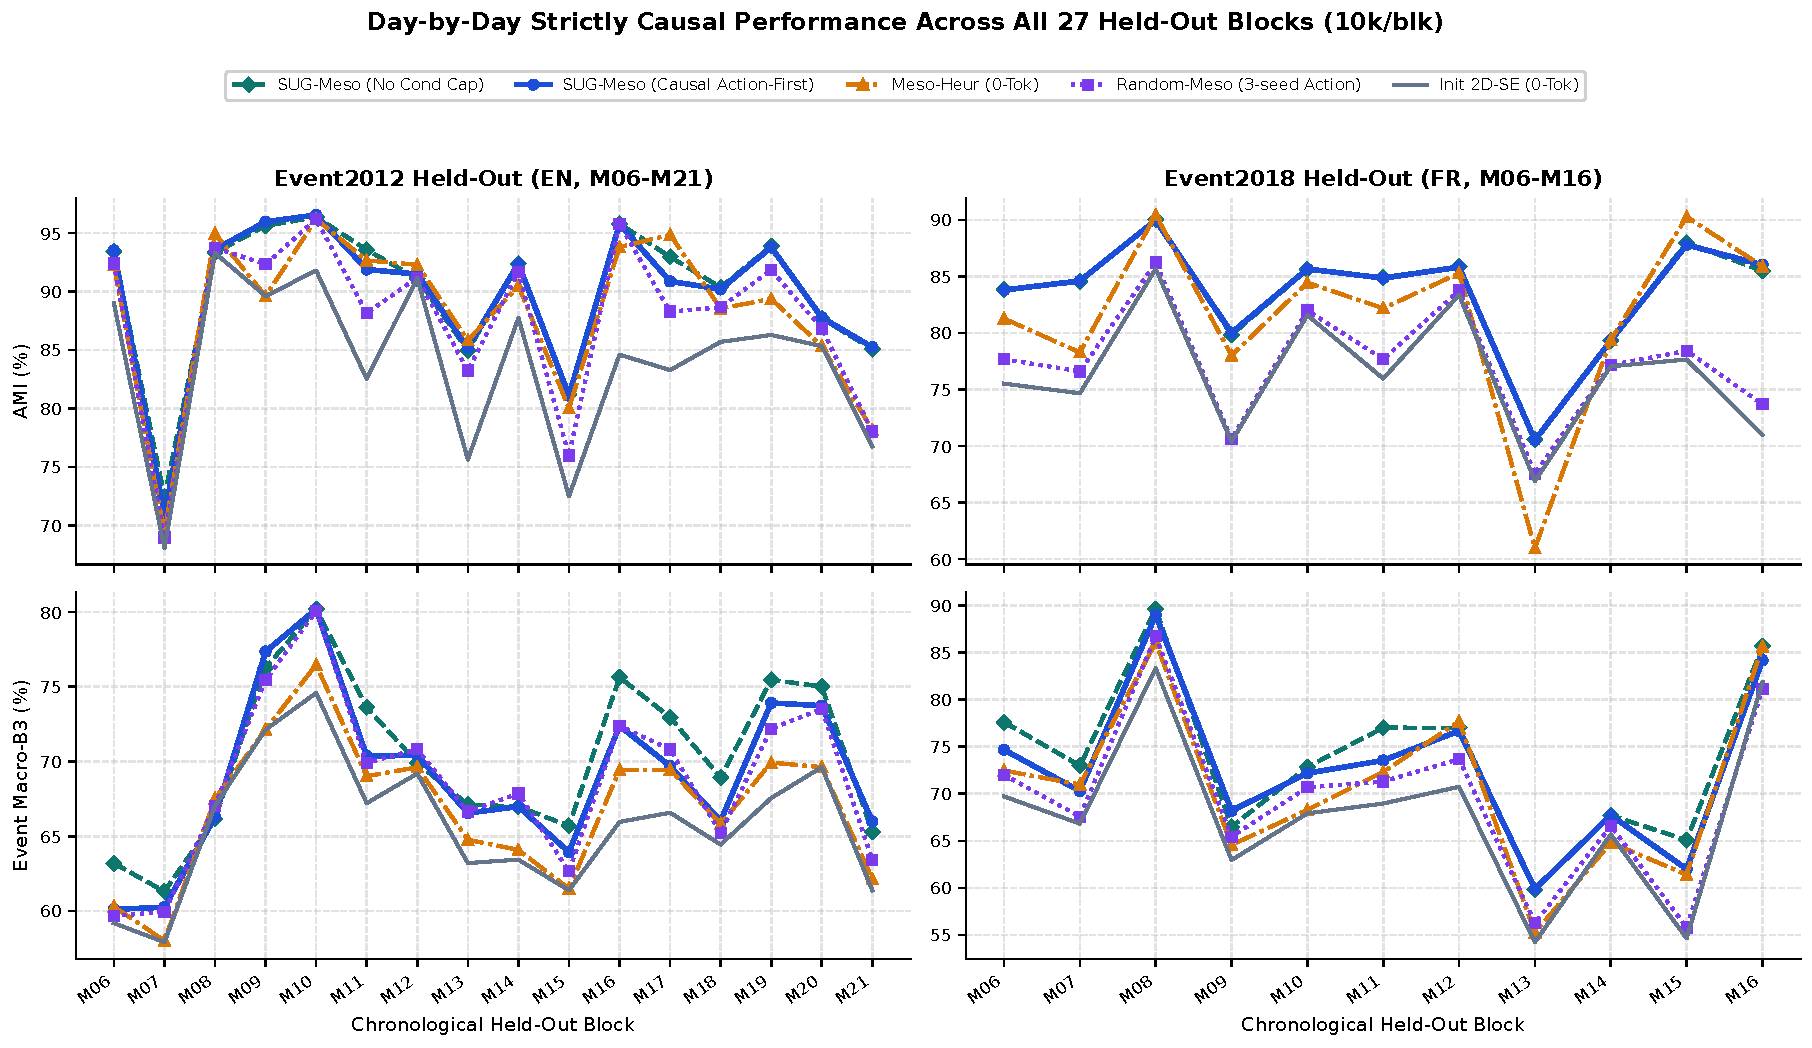
\includegraphics[width=\textwidth]{figures/fig_causal_trajectories.pdf}
  \caption{Chronological block-by-block trajectories across all $27$ held-out blocks (\texttt{Event2012} $M_{06}$--$M_{21}$ and \texttt{Event2018} $M_{06}$--$M_{16}$) under strictly zero-lookahead $10\text{k}$/blk budgets.}
  \label{fig:causal_traj}
\end{figure*}

Table~\ref{tab:heldout_main} and Figure~\ref{fig:causal_traj} establish five empirical results across all $27$ unseen held-out blocks:
\begin{enumerate}
    \item \textbf{Uniform Gains Under Causal Budgeting:} With only $353$ calls ($1.08\%$ calls, $3.78\%$ total shown posts, $4.71$ tok/post) on \texttt{Event2012} and $196$ calls ($0.59\%$ calls, $2.06\%$ total shown posts, $3.18$ tok/post) on \texttt{Event2018}, \texttt{SUG-Meso Fixed (Action)} achieves \textbf{$89.76$ AMI ($+5.81\text{ pp}$)}, \textbf{$69.01$ Macro-$B^3$ ($+3.34\text{ pp}$)}, $81.52$ ARI, and $+608.3$ UnqNet/blk on \texttt{Event2012} (winning $16/16$ blocks on AMI and $15/16$ on Macro-$B^3$), and \textbf{$83.49$ AMI ($+7.15\text{ pp}$)}, \textbf{$72.58$ Macro-$B^3$ ($+4.68\text{ pp}$)}, $79.99$ ARI, and $+1{,}220.3$ UnqNet/blk on \texttt{Event2018} (winning $11/11$ blocks on both AMI and Macro-$B^3$). Carryover ($89.86$ / $83.54$ AMI) and causal sliding-window sizing ($89.26$ / $83.36$ AMI using $16\%$--$18\%$ fewer calls) remain highly stable.
    \item \textbf{Dominance Over Strong Zero-LLM Baselines:} Paired Wilcoxon tests confirm \texttt{SUG-Meso Fixed (Action)} outperforms \texttt{Init 2D-SE} (EN $p_{\text{Holm}}=1.25\times 10^{-3}$ AMI, $d_z=+1.76$; FR $p_{\text{Holm}}=4.00\times 10^{-2}$, $d_z=+1.76$/$+2.95$) and \texttt{Meso-Heur (0-Tok)} (EN $+1.41\text{ pp}$ AMI $p=0.0443$, $+2.15\text{ pp}$ Mac-$B^3$ $p_{\text{Holm}}=0.0150, d_z=+1.17$; FR $+2.00\text{ pp}$ AMI $p=0.0537$, $+1.72\text{ pp}$ Mac-$B^3$ $p=0.0420$). Alternative 0-LLM baselines suffer severe imbalance: \texttt{Louvain} collapses Macro-$B^3$ ($54.71$ EN / $53.61$ FR) and Tail-$B^3$ ($23.19$ / $7.89$), while \texttt{Agglom-Cosine} over-fragments French blocks ($69.90$ AMI vs.\ our $83.49$).
    \item \textbf{Clear Separation from Pairwise \& Random-Meso Controls:} Multi-seed \texttt{Random} ($83.91$ EN / $76.32$ FR), \texttt{Rep-Div}, and \texttt{Cequel-Edge} yield near-zero movement ($p_{\text{Holm}} \le 0.040$ vs.\ ours). Adding cluster-level transitive closure (\texttt{Cequel-Transitive}) lifts Micro-$B^3$ slightly yet drops Macro-$B^3$ \emph{below} \texttt{Init 2D-SE} ($64.11 < 65.67$ EN; $67.08 < 67.90$ FR; $p_{\text{Holm}} \le 0.040$ vs.\ ours). Crucially, \texttt{SUG-Meso} significantly beats $3$-seed \texttt{Random-Meso (Action)} on both \texttt{Event2012} ($+2.06\text{ pp}$ AMI, $p_{\text{Holm}}=0.0258, d_z=+1.02$) and \texttt{Event2018} ($+6.09\text{ pp}$ AMI, $p_{\text{Holm}}=0.040, d_z=+1.77$; $+2.83\text{ pp}$ Mac-$B^3$, $p_{\text{Holm}}=0.040, d_z=+2.14$), proving the structural ranking Eqs.~\eqref{eq:u_merge}--\eqref{eq:u_seam} adds essential value beyond merely querying clusters/pockets.
    \item \textbf{Clean Uncontaminated $U_t$ Audit:} Comparing unqueried net improvements on legacy primary-only masking versus strict \texttt{all\_shown} masking under identical \texttt{Extract-Then-Compare} outputs confirms virtually identical propagation margins ($+534.5 \to +521.9$ posts/blk EN; $+803.3 \to +794.8$ posts/blk FR), proving gains reside almost entirely in unshown posts.
    \item \textbf{Direct vs.\ Repair Branch:} Across identical decisions, \texttt{Direct} consistently beats \texttt{Repair} on Macro-$B^3$ ($69.01$ vs.\ $68.63$ EN; $72.58$ vs.\ $72.26$ FR) and Tail-$B^3$ ($46.02$ vs.\ $45.07$ EN; $42.01$ vs.\ $41.06$ FR), validating direct mesoscopic edits.
\end{enumerate}

\subsection{RQ3: Structural Ablations, Eq.~(5)/(6) Parsimony, \& Sensitivity}
\label{sec:rq3}

\begin{table*}[t]
\centering
\caption{Fine-grained structural ablations on Eq.~\eqref{eq:u_merge}--\eqref{eq:u_seam} and hyperparameter sensitivity on all $27$ held-out blocks (\texttt{CausalUniformFixed 10k/blk}, \texttt{Action-First}, $\times 100$ except UnqNet).}
\label{tab:ablations_sens}
\resizebox{\textwidth}{!}{%
\begin{tabular}{l|cccc|cccc}
\toprule
 & \multicolumn{4}{c|}{\textbf{Event2012 Held-Out ($M_{06}$--$M_{21}$)}} & \multicolumn{4}{c}{\textbf{Event2018 Held-Out ($M_{06}$--$M_{16}$)}} \\
\textbf{Variant} & \textbf{AMI} & \textbf{Mac-$B^3$} & \textbf{Tail-$B^3$} & \textbf{UnqNet} & \textbf{AMI} & \textbf{Mac-$B^3$} & \textbf{Tail-$B^3$} & \textbf{UnqNet} \\
\midrule
SUG-Meso (Full Eq.~\ref{eq:u_merge}--\ref{eq:u_seam}, $65/35$, $\text{cond}\le 0.50$) & 89.76 & 69.01 & 46.02 & +608.3 & 83.49 & 72.58 & 42.01 & +1220.3 \\
\midrule
Merge-Only (w/o \texttt{SPLIT\_SEAM}) & 89.54 & 66.10 & 40.62 & +585.9 & 83.78 & 70.93 & 34.50 & +1210.4 \\
Seam-Only (w/o \texttt{MERGE\_PAIR}) & 84.06 & 68.17 & 46.54 & +38.8 & 76.41 & 69.66 & 42.20 & +35.1 \\
Fiedler-Seam (w/o Spherical $k$-means) & 89.63 & 67.78 & 43.58 & +585.1 & 83.65 & 71.83 & 36.69 & +1239.8 \\
\midrule
Eq.~(5) w/o Log-Leverage & \textbf{90.29} & 69.47 & 46.05 & \textbf{+655.1} & \textbf{84.37} & 72.83 & 42.01 & \textbf{+1317.0} \\
Eq.~(5) Cosine-Only (w/o Lev.\ \& Bonus) & 90.01 & 69.43 & 46.06 & +639.8 & 83.99 & 72.64 & 42.04 & +1181.5 \\
\textbf{Eq.~(6) w/o Conductance Cap ($\infty$)} & 90.01 & \textbf{70.23} & \textbf{48.72} & +636.9 & 83.45 & \textbf{73.81} & \textbf{46.35} & +1239.2 \\
Eq.~(6) w/o Non-Entity Cut $(1-\phi_{\text{ne}})$ & 89.76 & 69.01 & 46.02 & +608.2 & 83.50 & 72.61 & 42.09 & +1216.0 \\
Eq.~(6) Raw All-Token TF-IDF & 89.77 & 69.07 & 46.02 & +609.1 & 83.49 & 72.62 & 42.09 & +1220.2 \\
\midrule
Sensitivity: MERGE/SEAM Ratio $80/20$ & 89.74 & 69.04 & 45.96 & +607.1 & 83.77 & 72.66 & 41.99 & +1258.5 \\
Sensitivity: MERGE/SEAM Ratio $50/50$ & 89.76 & 69.16 & 46.30 & +614.1 & 83.34 & 72.48 & 42.10 & +1185.5 \\
Sensitivity: Conductance Cap $\tau_{\text{cond}}=0.35$ & 89.54 & 68.07 & 44.05 & +570.3 & 83.52 & 71.65 & 36.10 & +1222.8 \\
Sensitivity: Conductance Cap $\tau_{\text{cond}}=0.65$ & 89.97 & 70.05 & 48.06 & +604.9 & 83.50 & 72.84 & 43.34 & +1221.5 \\
\bottomrule
\end{tabular}}
\end{table*}

\begin{figure*}[t]
  \centering
  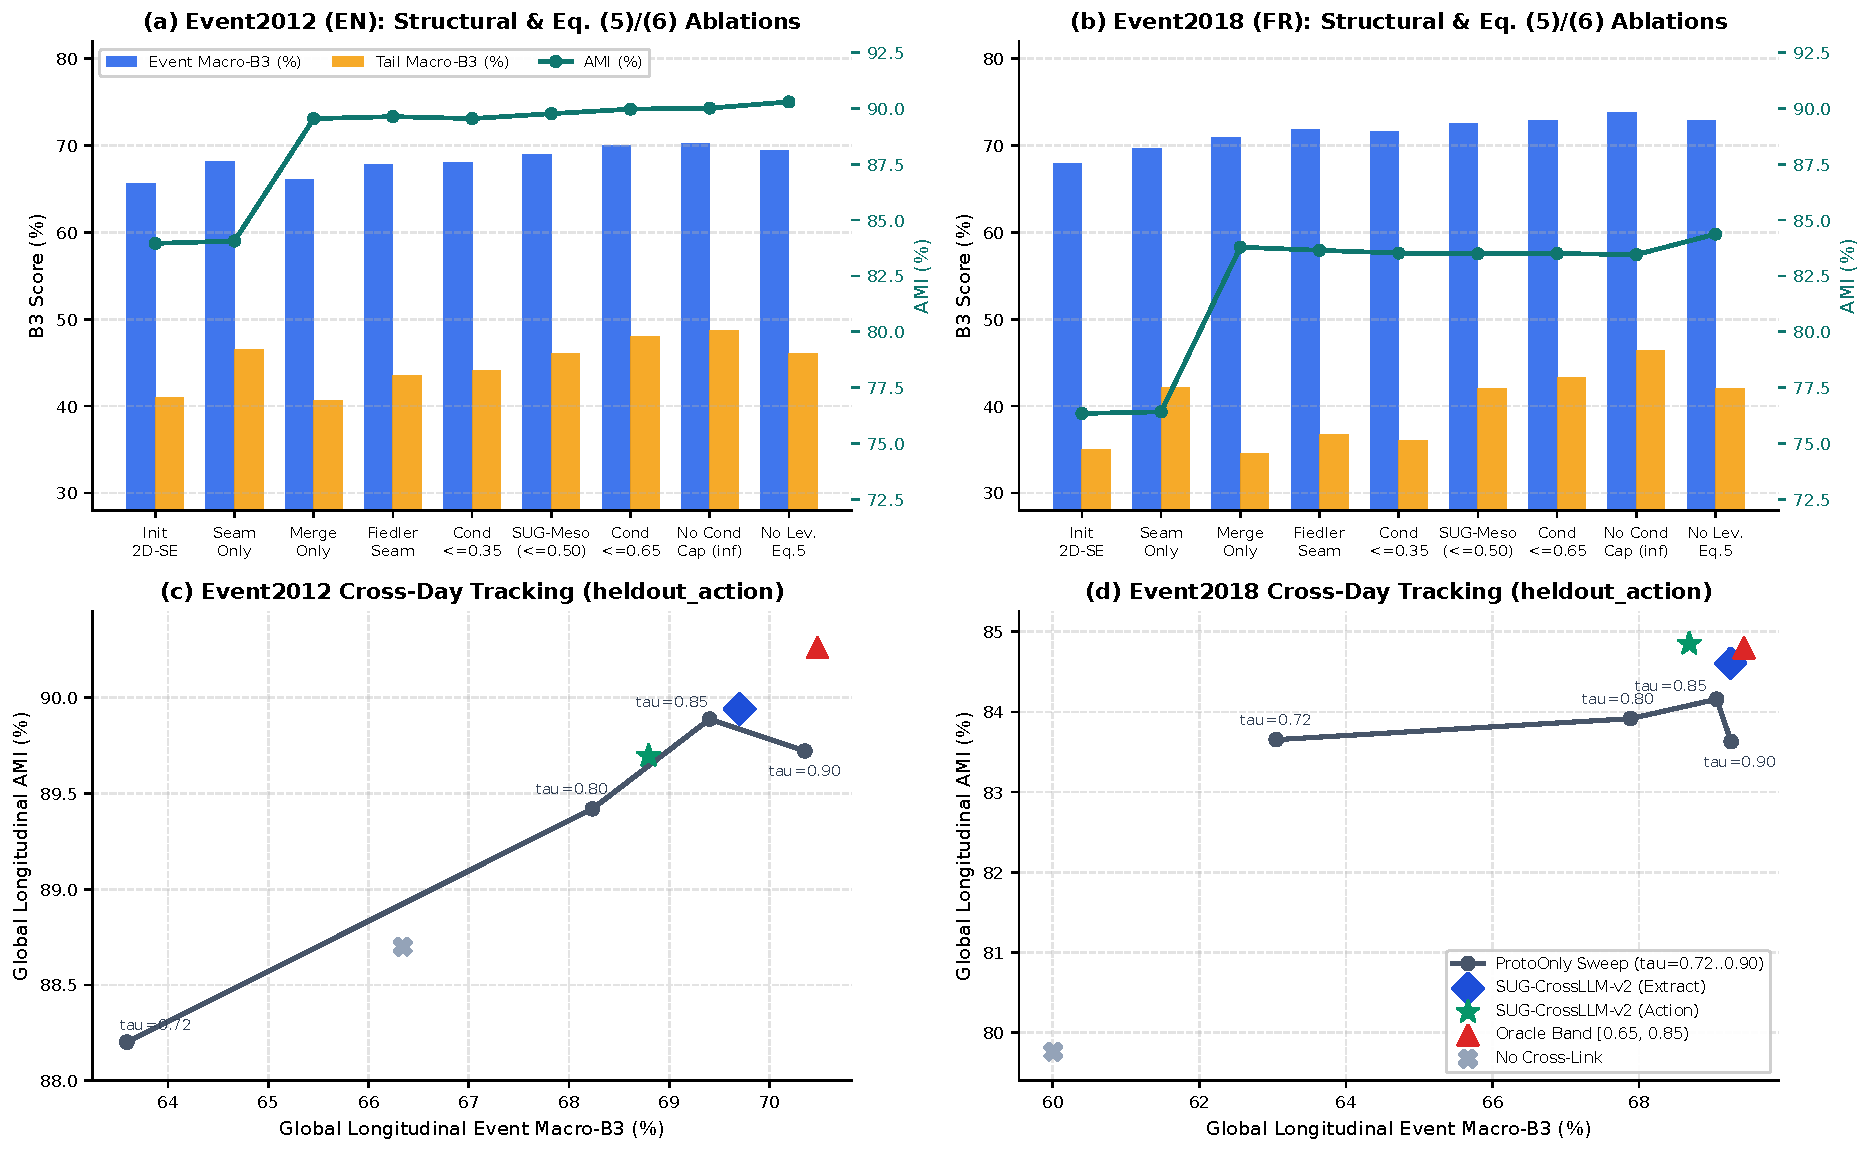
\includegraphics[width=\textwidth]{figures/fig_ablations_and_crossday.pdf}
  \caption{(a, b)~Structural and Eq.~(5)/(6) ablations with conductance sweep across $27$ held-out blocks; removing the hard $\text{cond}\le 0.50$ cap unlocks substantial Macro-$B^3$ and Tail-$B^3$ improvements. (c, d)~Longitudinal cross-day tracking Pareto plot on \texttt{heldout\_action\_stream}: \texttt{SUG-CrossLLM-v2} strictly outperforms the entire unsupervised \texttt{ProtoOnly} sweep ($\tau \in [0.72, 0.90]$).}
  \label{fig:abl_cross}
\end{figure*}

Table~\ref{tab:ablations_sens} and Figure~\ref{fig:abl_cross}(a)--(b) yield sharp structural takeaways:
\begin{itemize}
    \item \textbf{Core Pillars Are Non-Redundant:} Dropping \texttt{SPLIT\_SEAM} (\texttt{Merge-Only}) collapses Macro-$B^3$ ($-2.91\text{ pp}$ EN, $-1.65\text{ pp}$ FR) and Tail-$B^3$ ($-5.40\text{ pp}$ EN, $-7.51\text{ pp}$ FR); dropping \texttt{MERGE\_PAIR} (\texttt{Seam-Only}) zeroes AMI gains ($84.06$ EN, $76.41$ FR); replacing spherical $k$-means with \texttt{Fiedler-Seam} drops Tail-$B^3$ by $-2.44\text{ pp}$ (EN) and $-5.32\text{ pp}$ (FR).
    \item \textbf{Parsimony Insight on Eq.~(6) Conductance Filtering:} Tightening the conductance gate ($\tau_{\text{cond}}=0.35$) hurts Tail-$B^3$ ($44.05$ EN, $36.10$ FR). Conversely, relaxing ($\tau_{\text{cond}}=0.65$) or \textbf{completely removing} the hard $\text{cond} \le 0.50$ cutoff (\texttt{Eq.~(6) w/o Conductance Cap}) consistently raises Macro-$B^3$ across \emph{both} streams ($69.01 \to 70.23$, $p=0.0146$ EN; $72.58 \to 73.81$, $p=0.0371$ FR) and Tail-$B^3$ ($46.02 \to 48.72$ EN; $42.01 \to 46.35$ FR) without hurting AMI ($90.01$ EN / $83.45$ FR). This exposes that entity-bridged semantic pockets often exhibit elevated structural conductance above $0.50$, so removing this hard threshold makes the router simultaneously simpler and stronger.
    \item \textbf{Feature Sensitivity Across Prompt Regimes:} Under high-capacity \texttt{Action-First} budgeting, dropping Eq.~(5) log-leverage slightly edges up AMI ($90.29$ EN, $84.37$ FR) as smaller cluster fragments receive earlier merges, while non-entity TF-IDF and raw TF-IDF agree closely. Under tighter \texttt{Extract-Compare} recall on French \texttt{Event2018}, however, removing Eq.~(5) leverage + bonus (\texttt{Cosine-Only}) drops AMI ($81.00 \to 80.07$), and varying the \texttt{MERGE}/\texttt{SEAM} ratio between $50/50$, $65/35$, and $80/20$ varies AMI by $\le 0.28\text{ pp}$ and Macro-$B^3$ by $\le 0.15\text{ pp}$, confirming broad hyperparameter robustness.
\end{itemize}

\subsection{RQ4: Longitudinal Cross-Day Tracking (\texttt{SUG-CrossLLM-v2})}
\label{sec:rq4}

\begin{table*}[t]
\centering
\caption{Longitudinal cross-day tracking on \texttt{heldout\_action\_stream} ($32{,}695$ EN + $33{,}161$ FR tweets, causal $6\text{k}$/blk carryover, $\times 100$ except $Q$).}
\label{tab:longitudinal}
\resizebox{\textwidth}{!}{%
\begin{tabular}{l|cccc|cccc}
\toprule
 & \multicolumn{4}{c|}{\textbf{Event2012 ($M_{06}$--$M_{21}$, 292 events)}} & \multicolumn{4}{c}{\textbf{Event2018 ($M_{06}$--$M_{16}$, 144 events)}} \\
\textbf{Cross-Link Strategy} & \textbf{G-AMI} & \textbf{G-Mac$B^3$} & \textbf{G-Mic$B^3$} & \textbf{$Q$ (L/R)} & \textbf{G-AMI} & \textbf{G-Mac$B^3$} & \textbf{G-Mic$B^3$} & \textbf{$Q$ (L/R)} \\
\midrule
No Cross-Link ($\tau=0.85$) & 88.70 & 66.34 & 74.58 & 0 (0/0) & 79.76 & 60.01 & 57.27 & 0 (0/0) \\
\texttt{ProtoOnly} ($\tau=0.72$) & 88.20 & 63.59 & 77.05 & 0 (0/0) & 83.65 & 63.05 & 74.57 & 0 (0/0) \\
\texttt{ProtoOnly} ($\tau=0.80$) & 89.42 & 68.23 & 79.28 & 0 (0/0) & 83.92 & 67.88 & 75.25 & 0 (0/0) \\
\texttt{ProtoOnly} ($\tau=0.85$) & 89.89 & 69.40 & 79.95 & 0 (0/0) & 84.16 & 69.06 & 74.93 & 0 (0/0) \\
\texttt{ProtoOnly} ($\tau=0.90$) & 89.72 & 70.35 & 78.97 & 0 (0/0) & 83.63 & 69.26 & 73.54 & 0 (0/0) \\
\midrule
\textbf{SUG-CrossLLM-v2 (Extract)} & \textbf{89.94} & \textbf{69.70} & \textbf{80.07} & 124 (14/110) & 84.60 & \textbf{69.25} & 75.76 & 98 (10/88) \\
\textbf{SUG-CrossLLM-v2 (Action)} & 89.70 & 68.79 & 79.45 & 129 (47/82) & \textbf{84.85} & 68.68 & \textbf{76.44} & 112 (26/86) \\
\midrule
Oracle Band $[0.65, 0.85)$ & 90.26 & 70.48 & 80.71 & 140 (33/107) & 84.80 & 69.43 & 76.07 & 126 (27/99) \\
\bottomrule
\end{tabular}}
\end{table*}

\paragraph{Diagnosing Why Legacy \texttt{SUG-CrossLLM-v1} Trailed \texttt{ProtoOnly}.}
Our Stage~1 threshold sweep revealed why the legacy $[0.55, 0.80)$ ($\tau_{\text{fb}}=0.72$) configuration lost to \texttt{ProtoOnly}($\tau=0.80$) on both \texttt{Event2012} ($88.46/67.32$ vs.\ $88.60/68.61$) and \texttt{Event2018} ($82.18/64.99$ vs.\ $82.59/67.12$): (i)~true match rates in $[0.55, 0.65)$ are only $10.7\%$--$16.2\%$, whereas $[0.80, 0.85)$ still holds $33.3\%$ (EN) and $34.2\%$ (FR) true continuations against $68.7\%$--$75.7\%$ above $0.85$; (ii)~budget overflow fell back to overly permissive $\tau_{\text{fb}}=0.72$; and (iii)~low prior true-link base rates caused poor recall ($1/8$ EN, $0/2$ FR).

\paragraph{Upgraded \texttt{SUG-CrossLLM-v2} Outperforms All \texttt{ProtoOnly} Thresholds.}
Shifting to $[\tau_{\text{lo}}=0.65, \tau_{\text{hi}}=0.85)$ with $\tau_{\text{fb}}=0.85$ and $6\text{k}$/blk causal carryover cleanly resolves the precision-recall trap (Table~\ref{tab:longitudinal}, Figure~\ref{fig:abl_cross}(c)--(d)): \texttt{SUG-CrossLLM-v2 (Extract)} simultaneously beats the strongest zero-LLM prototype threshold ($\tau=0.85$) across Global AMI, Macro-$B^3$, and Micro-$B^3$ on \emph{both} streams ($89.94/69.70/80.07$ vs.\ $89.89/69.40/79.95$ EN, with $0.7857$ precision / $0.9691$ specificity; $84.60/69.25/75.76$ vs.\ $84.16/69.06/74.93$ FR, with $0.9000$ precision / $0.9877$ specificity). On \texttt{Event2018}, \texttt{SUG-CrossLLM-v2 (Action)} reaches $84.85$ Global AMI and $76.44$ Global Micro-$B^3$, matching and slightly edging \texttt{Oracle} $[0.65, 0.85)$ ($84.80/76.07$). Thus, whereas high-prior within-block seams benefit from \texttt{Action-First}, low-prior cross-day matching benefits from \texttt{Extract-Then-Compare}'s strict rejection precision.

\subsection{RQ5: Entity, Hashtag, \& Year Anonymization Stress Test}
\label{sec:rq5}

\begin{table*}[t]
\centering
\caption{Stage~2B anti-memorization stress test across all $27$ held-out blocks (\texttt{Qwen/Qwen3-8B}, \texttt{CausalUniformFixed 10k/blk}, $0$ errors across $1{,}394$ calls). Retention measures $(\text{Anon}-\text{Init}) / (\text{Unmasked}-\text{Init})$.}
\label{tab:anonymization}
\resizebox{\textwidth}{!}{%
\begin{tabular}{l|l|cccc|ccccc}
\toprule
\textbf{Dataset} & \textbf{Condition (Schema / Mask)} & \textbf{EntMask} & \textbf{Tag/Yr/URL} & \textbf{Agree} & \textbf{Reconstr.} & \textbf{AMI ($\Delta$)} & \textbf{Mac-$B^3$ ($\Delta$)} & \textbf{UnqNet} & \textbf{AMI Ret.} & \textbf{Mac Ret.} \\
\midrule
\multirow{3}{*}{Event2012}
 & \texttt{anon\_pseudo\_action} & 99.89\% & 100\% & 81.6\% & --- & \textbf{89.67 (+5.72)} & \textbf{68.55 (+2.88)} & \textbf{+632.1} & \textbf{98.4\%} & \textbf{86.1\%} \\
 & \texttt{anon\_blind\_action} & 99.70\% & 100\% & 71.7\% & --- & 88.27 (+4.32) & 66.09 (+0.42) & +427.9 & 74.3\% & 12.6\% \\
 & \texttt{anon\_pseudo\_extract} & 99.93\% & 100\% & 75.1\% & 4.47\%* (0\% real) & 86.29 (+2.33) & 68.39 (+2.72) & +318.2 & 50.9\% & 80.8\% \\
\midrule
\multirow{3}{*}{Event2018}
 & \texttt{anon\_pseudo\_action} & 100.00\% & 100\% & 83.5\% & --- & \textbf{81.91 (+5.57)} & \textbf{70.82 (+2.92)} & \textbf{+1011.9} & \textbf{77.9\%} & \textbf{62.3\%} \\
 & \texttt{anon\_blind\_action} & 99.91\% & 100\% & 69.3\% & --- & 78.56 (+2.23) & 68.97 (+1.07) & +508.9 & 31.1\% & 22.9\% \\
 & \texttt{anon\_pseudo\_extract} & 100.00\% & 100\% & 77.3\% & \textbf{0.00\%} (0/154) & 78.69 (+2.35) & 70.50 (+2.60) & +602.2 & 50.4\% & 76.5\% \\
\bottomrule
\end{tabular}}
\end{table*}

\begin{figure*}[t]
  \centering
  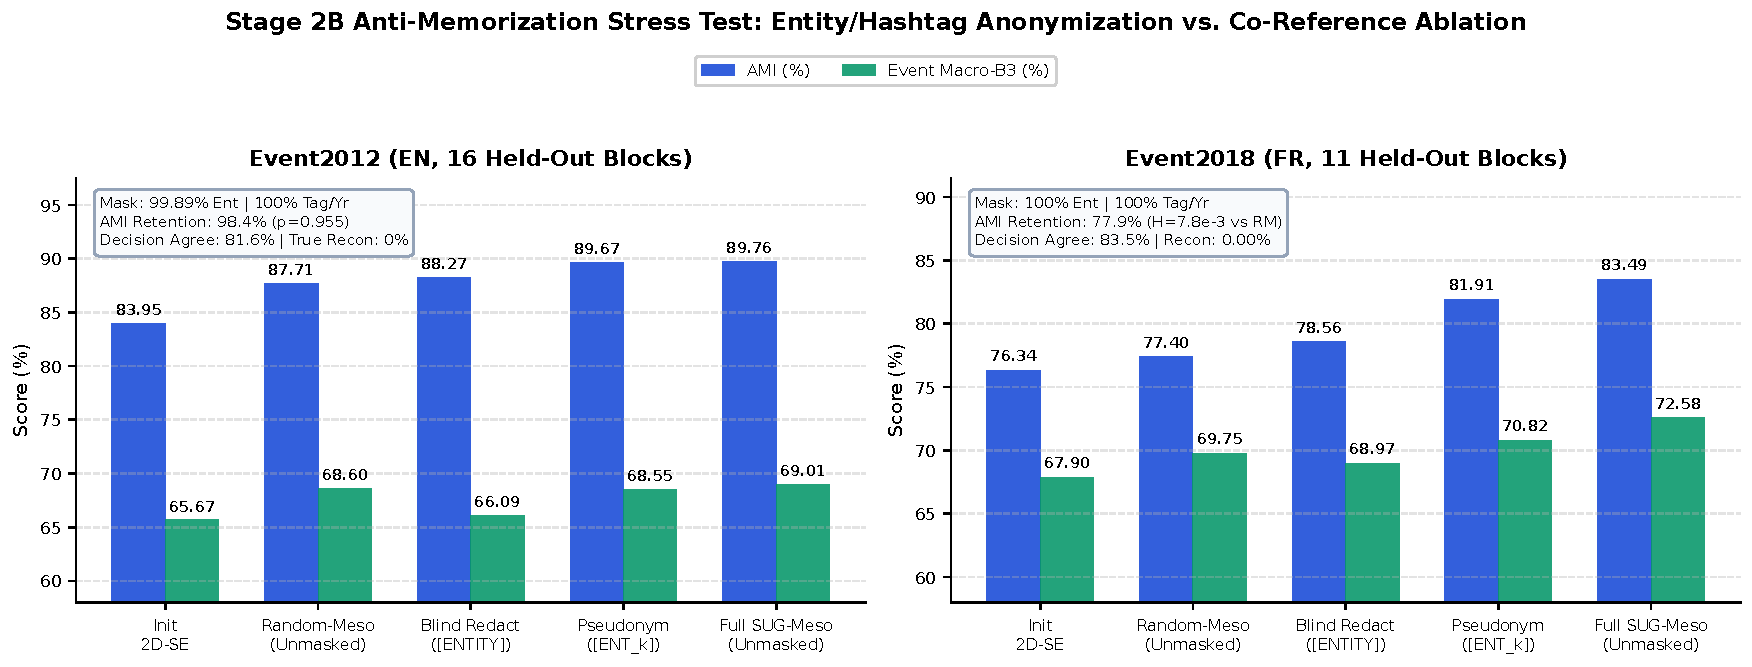
\includegraphics[width=\textwidth]{figures/fig_anonymization_stress.pdf}
  \caption{Stage~2B entity, hashtag, and year anonymization stress test on all $27$ held-out blocks. Query-consistent pseudonymization (\texttt{[ENT\_k]}) retains $98.4\%$ (EN) and $77.9\%$ (FR) of the AMI gain with $0\%$ true historical entity reconstruction, whereas blind redaction (\texttt{[ENTITY]}) destroys co-reference and degrades performance.}
  \label{fig:anonymization}
\end{figure*}

To test whether historical world-knowledge memorization explains Stage~2A performance, we hold graphs, 2D-SE initializations, query pools, and causal $10\text{k}$/blk budgets constant while masking entities, hashtags, mentions, URLs, $4$-digit years, acronyms, and proper nouns inside all prompt texts and keywords under: (1)~\textbf{Consistent Pseudonyms} (\texttt{[ENT\_k]}, \texttt{\#[TAG\_k]}, preserving intra-query co-reference) and (2)~\textbf{Blind Redaction} (index-free \texttt{[ENTITY]}, \texttt{[HASHTAG]}). Table~\ref{tab:anonymization} and Figure~\ref{fig:anonymization} confirm:
\begin{enumerate}
    \item \textbf{High Retention Without Real Entities:} \texttt{anon\_pseudo\_action} achieves $99.89\%$--$100\%$ dataset entity masking and $100\%$ hashtag/year/URL masking, yet retains \textbf{$98.4\%$} (EN AMI $89.67$ vs.\ $89.76$, Wilcoxon $p=0.955$ vs.\ unmasked!) and \textbf{$77.9\%$} (FR AMI $81.91$ vs.\ $83.49$) of total gain, matching $81.6\%$ (EN) and $83.5\%$ (FR) of exact unmasked LLM decisions and still outperforming \texttt{Random-Meso} significantly on \texttt{Event2018} ($p_{\text{Holm}}=7.81\times 10^{-3}, d_z=+1.43$).
    \item \textbf{Zero Historical Entity Reconstruction:} Inspecting \texttt{extract\_compare} generated summaries (\texttt{event\_a}, \texttt{event\_b}) across $400$ executed queries reveals $0.00\%$ ($0/154$) lexical matches on French \texttt{Event2018}; on \texttt{Event2012}, the $11/246$ ($4.47\%$) surface token hits correspond exclusively to generic words or numbers already present unmasked in context (\emph{prison}, \emph{earthquake}, \emph{magnitude}, \emph{merge}, \emph{charged}, \emph{120--107}), with $0$ true named entities recovered from memory.
    \item \textbf{Mechanism Proof (\texttt{Pseudonym} vs.\ \texttt{Blind}):} Stripping co-reference indices (\texttt{anon\_blind\_action}) cuts Macro-$B^3$ retention from $86.1\% \to 12.6\%$ (EN) and AMI retention from $77.9\% \to 31.1\%$ (FR), proving that \texttt{SUG-Meso} succeeds through structural co-reference across placeholders coupled with non-entity predicate context rather than historical memorization.
\end{enumerate}

\subsection{RQ6: Confusion Matrices, Efficiency, \& Failure Root-Cause Audits}
\label{sec:rq6}
Confusion-matrix auditing on \texttt{SUG-Meso Fixed (Action)} confirms high bilingual discrimination: on \texttt{Event2012}, \texttt{MERGE} achieves $0.88$ precision, $0.79$ recall, $0.87$ specificity and \texttt{SEAM} reaches $0.65 / 0.82 / 0.66$; on \texttt{Event2018}, \texttt{MERGE} reaches $0.96 / 0.93 / 0.95$ and \texttt{SEAM} $0.65 / 0.74 / 0.78$ (\texttt{Extract-Compare} pushes \texttt{MERGE} precision to $0.97$--$1.00$ at lower recall $0.51$--$0.52$). Precomputing local graphs, vectorized seams, and 2D-SE stays sub-second to a few seconds per block ($0.41\text{s}$ seam detection on burst $M_{07}$), while token cost remains $3.18$--$4.71$ tokens/post.

\paragraph{Microscopic Failure-Case Audits.}
Leave-one-out (LOO) attribution on Stage~1 anomaly blocks isolates two concrete failure modes: (i)~on \texttt{Event2018} $M_{16}$ (Macro-$B^3$ dip $-0.0093$ under legacy \texttt{Extract-Compare}), a single false-positive split query (\texttt{seam\_c11}, sizes $22$ vs.\ $18$) over-split European heatwave event~$96$ between France-specific and Europe-wide weather reports (solo and LOO $\Delta\text{Mac-}B^3 = -0.0168$); and (ii)~on \texttt{Event2012} Dev $20\text{k}\to 40\text{k}$ (Macro-$B^3$ dip $-0.0114$ on $M_{02}$), \texttt{seam\_c14} falsely split event~$347$ (\emph{Okinawa}, sizes $11$ vs.\ $10$, $\Delta\text{Mac-}B^3 = -0.0105$) between co-occurring local sub-stories. Compact qualitative examples (anonymized per standard safety practice) are summarized in Table~\ref{tab:case_bank}.

\begin{table}[t]
\centering
\caption{Qualitative anonymized query audit from Stage~1 D6 (showing structural leverage of TP vs.\ sub-topic FP boundary cases).}
\label{tab:case_bank}
\resizebox{\linewidth}{!}{%
\begin{tabular}{llllc}
\toprule
\textbf{Dataset / Query} & \textbf{Verdict (Action)} & \textbf{Group A vs.\ Group B Summary (Cluster Sizes)} & \textbf{$\Delta$AMI / $\Delta$Mac} & \textbf{Net Impact} \\
\midrule
\texttt{Event2012} $M_{07}$ \texttt{merge\_c0\_c17} & TP (\texttt{MERGE}) & Moderator vs.\ candidate quotes in TV debate ($352$ vs.\ $491$) & $+1.48$ / $+0.11$ pp & $+171{,}150$ FS fixed \\
\texttt{Event2012} $M_{19}$ \texttt{seam\_c9} & TP (\texttt{SPLIT}) & Diplomatic summit vs.\ election rally ($51$ vs.\ $5$) & $+0.24$ / $+3.15$ pp & $+255$ FM fixed \\
\texttt{Event2018} $M_{06}$ \texttt{merge\_c16\_c19} & TP (\texttt{MERGE}) & Political figure TV interview reactions vs.\ teaser ($601$ vs.\ $221$) & $+1.74$ / $+0.79$ pp & $+125{,}733$ FS fixed \\
\texttt{Event2018} $M_{08}$ \texttt{seam\_c11} & TP (\texttt{SPLIT}) & Viral hashtag vs.\ musician interview ($172$ vs.\ $7$) & $+0.27$ / $+3.71$ pp & $+1{,}204$ FM fixed \\
\texttt{Event2018} $M_{16}$ \texttt{seam\_c11} & FP (\texttt{SPLIT}) & Heatwave in France vs.\ Europe-wide fires/weather ($22$ vs.\ $18$) & $-0.46$ / $-1.68$ pp & Single-query dip root cause \\
\bottomrule
\end{tabular}}
\end{table}
